 \documentclass[../ManualeSviluppatore_v1.0.0.tex]{subfiles}

\begin{document}

\section{Atavi::FrontEnd}

	\begin{figure}[!h]
		\centering
		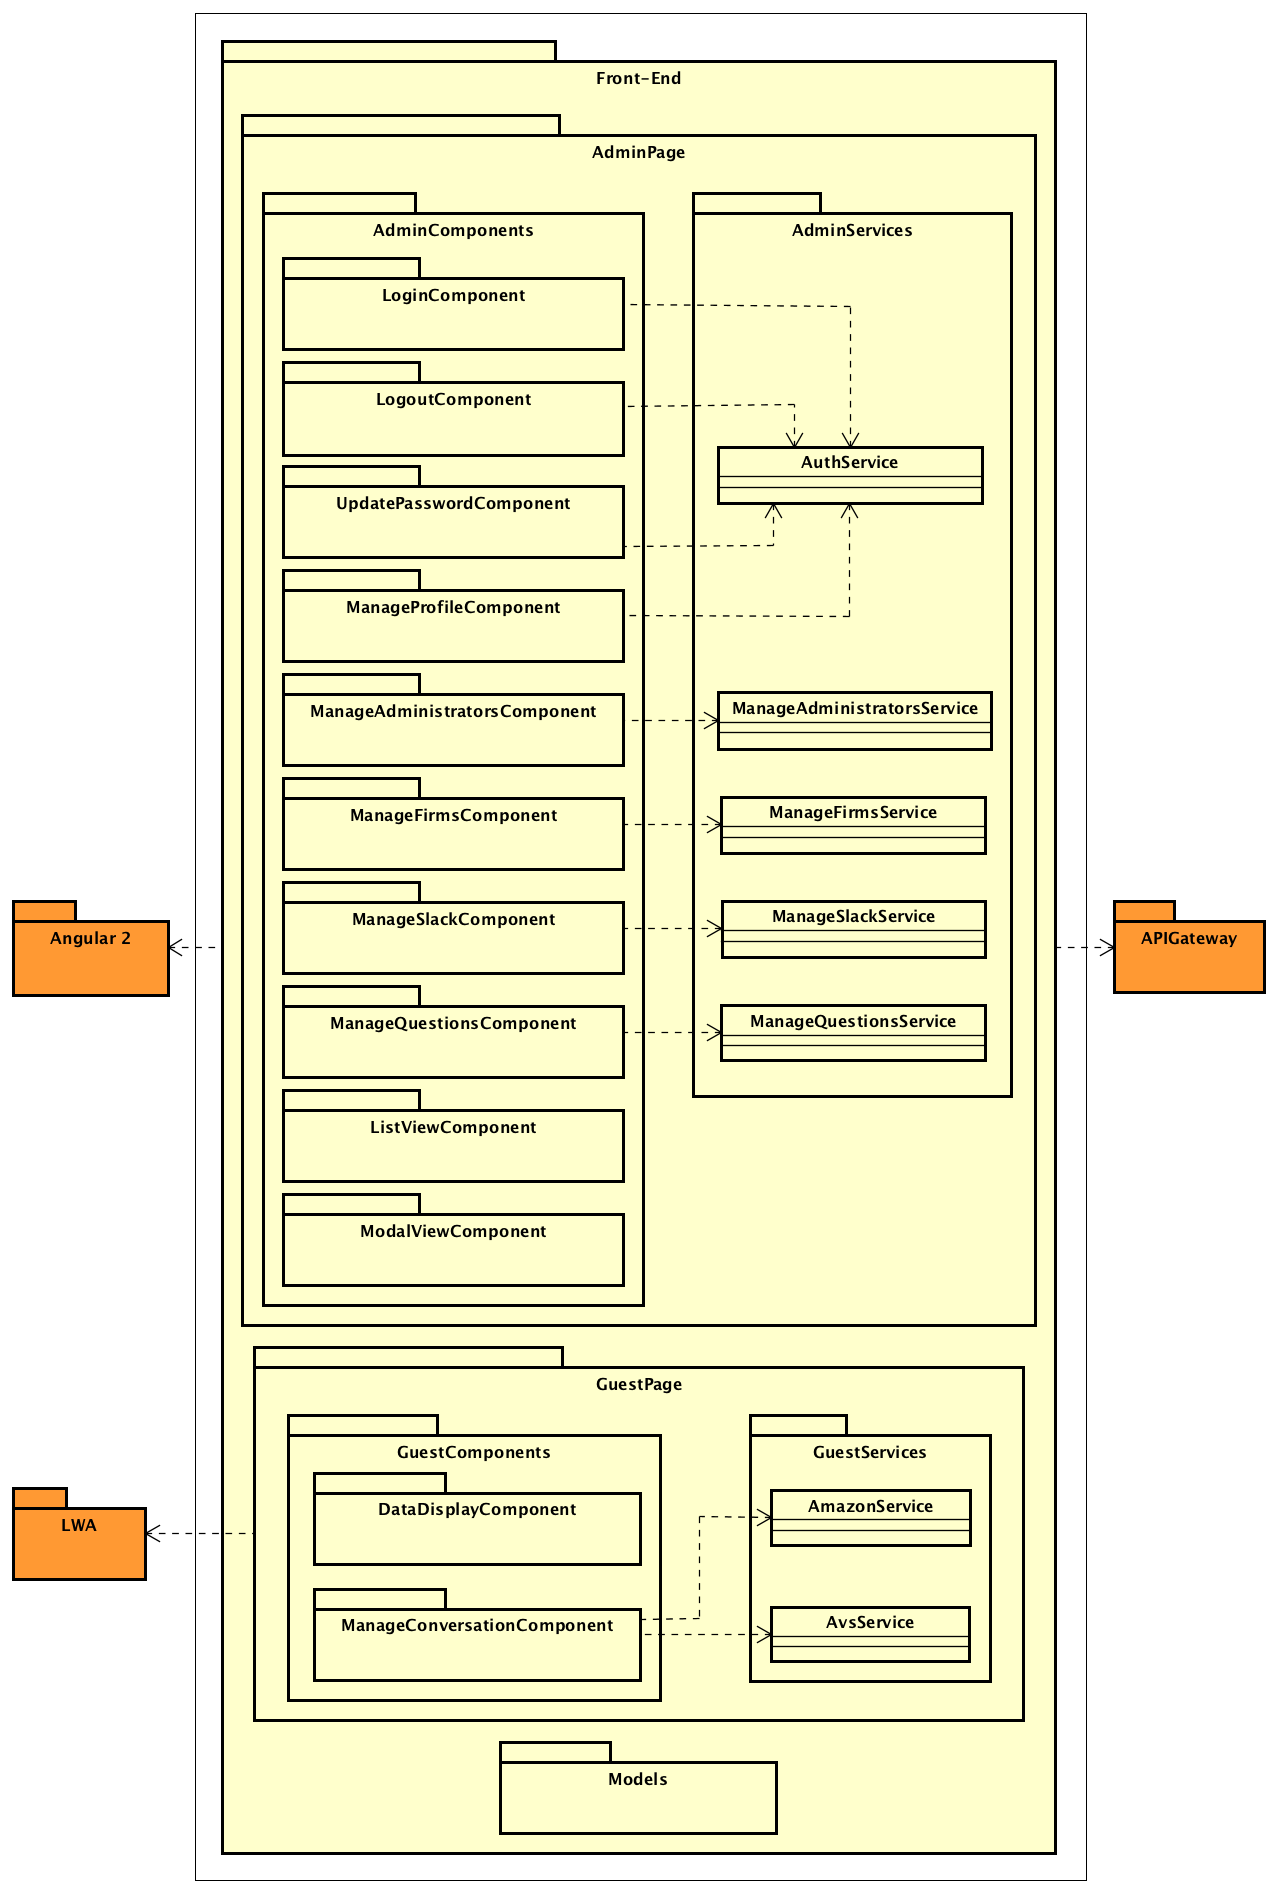
\includegraphics[scale=0.3]{Architettura/Front-end.png}
		\caption{Schema del componente \texttt{Front-End - Schema Generale}}
	\end{figure}
	\subparagraph{Descrizione}: Package che rappresenta il client dell'applicazione
	\subparagraph{Package contenuti}:
	\begin{itemize}
		\item Front-End :: AdminPage: Package dedicato alla parte client dell'Admin e del SuperAdmin;
		\item Front-End :: GuestPage: Package dedicato alla parte d'interfaccia client disponibile per l'ospite e per l'utente.
	\end{itemize}

	\newpage
	\subsection{Front-End :: AdminPage}
	\begin{figure}[!h]
		\centering
		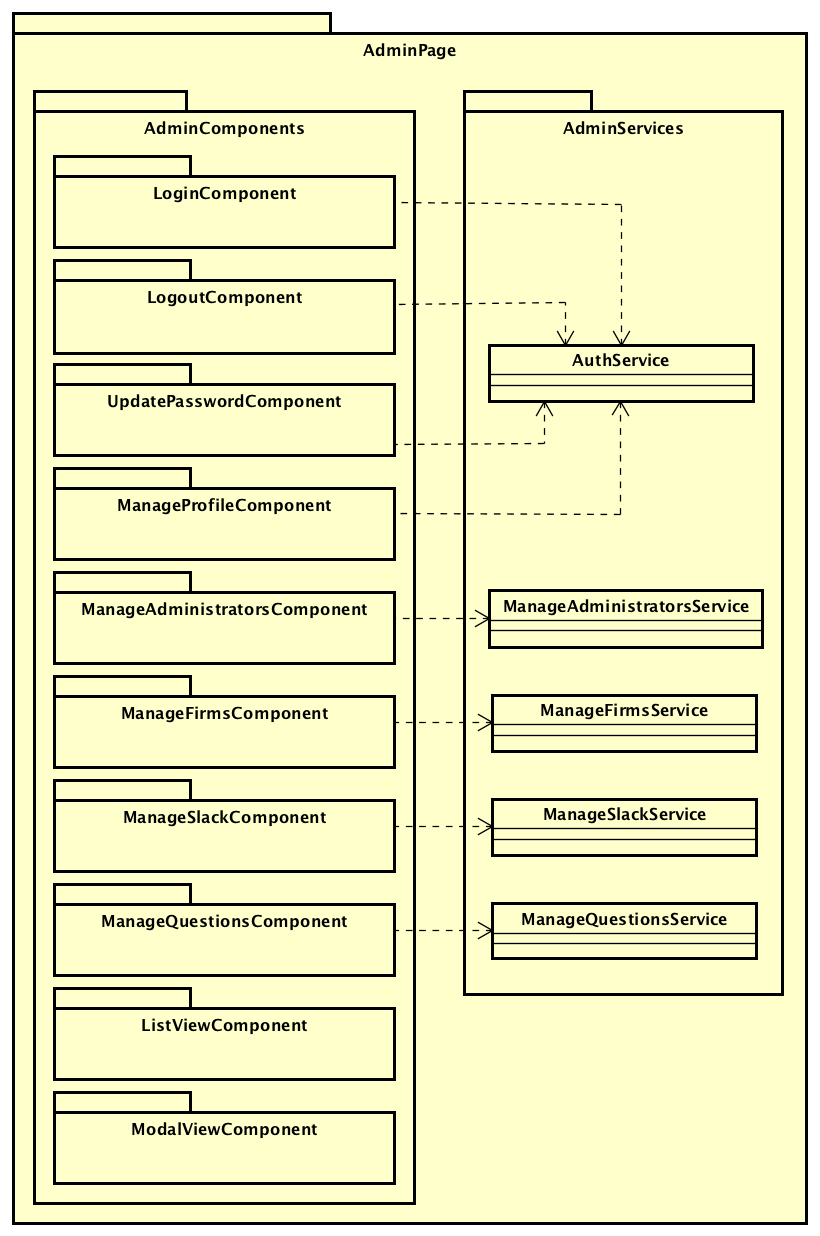
\includegraphics[scale=0.3]{Architettura/Front-End/AdminPage/AdminPage.png}
		\caption{Schema del componente \texttt{Front-End :: AdminPage}}
	\end{figure}
			\subparagraph{Descrizione}: Package dedicato alla parte client fruibile da un amministratore
			\subparagraph{Padre}: Front-End
			\subparagraph{Package contenuti}:
			\begin{itemize}
				\item AdminPage :: AdminComponents: Package contenente tutti i componenti necessari al Front-End della console amministrativa, comprensivi quindi dei models che andranno ad utilizzare e delle relative view e controller;
				\item AdminPage :: AdminServices: Package che fornisce tutti i servizi utilizzabili dai componenti presenti in AdminComponents.
			\end{itemize}

	\subsection{Front-End :: AdminPage :: AdminComponents}

		\subparagraph{Descrizione}: Classe contenente tutti i metodi necessari a gestire il Front-End della console amministrativa
		\subparagraph{Padre}: AdminPage
		\subparagraph{Package contenuti}:
		\begin{itemize}
			\item AdminPage :: AdminComponents :: LoginComponent: Componente che contiene al suo interno la sua view, il suo controller, ed i models di cui necessita
			\item AdminPage :: AdminComponents :: LogoutComponent: Componente che contiene al suo interno la sua view, il suo controller, ed i models di cui necessita
			\item AdminPage :: AdminComponents :: ManageAdministratorsComponent: Componente che contiene al suo interno la sua view, il suo controller, ed i models di cui necessita
			\item AdminPage :: AdminComponents :: ManageFirmsComponent: Componente che contiene al suo interno la sua view, il suo controller, ed i models di cui necessita
			\item AdminPage :: AdminComponents :: ManageProfileComponent: Componente che contiene al suo interno la sua view, il suo controller, ed i models di cui necessita
			\item AdminPage :: AdminComponents :: ManageQuestionsComponent: Componente che contiene al suo interno la sua view, il suo controller, ed i models di cui necessita
			\item AdminPage :: AdminComponents :: ManageSlackComponent: Componente che contiene al suo interno la sua view, il suo controller, ed i models di cui necessita
			\item AdminPage :: AdminComponents :: UpdatePasswordComponent: Componente che contiene al suo interno la sua view, il suo controller, ed i models di cui necessita
			\item AdminPage :: AdminComponents :: ListViewComponent: Componente che contiene al suo interno la sua view, il suo controller, ed i models di cui necessita
			\item AdminPage :: AdminComponents :: ModalViewComponent: Componente che contiene al suo interno la sua view, il suo controller, ed i models di cui necessita
		\end{itemize}

\newpage
	\subsection{Front-End :: AdminPage :: AdminComponents :: LoginComponent}
	\begin{figure}[!h]
		\centering
		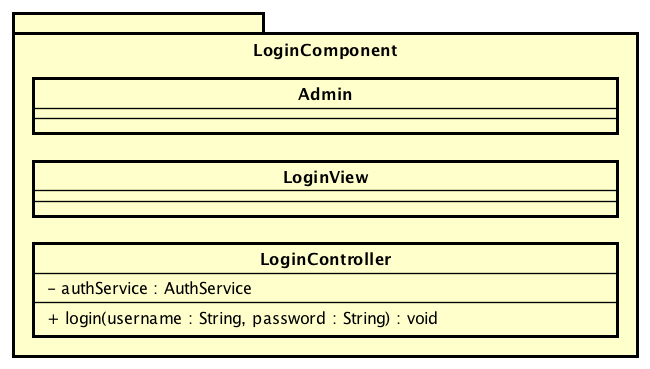
\includegraphics[scale=0.6]{Architettura/Front-End/AdminPage/AdminComponents/LoginComponent.png}
		\caption{Schema del componente \texttt{Front-End :: AdminPage :: AdminComponents :: LoginComponent}}
	\end{figure}
			\subparagraph{Descrizione}: Componente che contiene al suo interno la sua view, il suo controller, ed i models di cui necessita
			\subparagraph{Padre}: AdminComponents
			\subsubsection{Front-End :: AdminPage :: AdminComponents :: LoginComponent :: LoginController}
				\subparagraph{Descrizione}: Controller che gestisce la view di LoginView permettendo ad un amministratore di effettuare l'accesso alla console amministrativa
				\subparagraph{Costanti}:
				\begin{itemize}
					\item \texttt{authService: AuthService}: Attributo che rappresenta una istanza del service AuthService e ne mette a disposizione i metodi.
				\end{itemize}
	  		\subsubsection{Front-End :: AdminPage :: AdminComponents :: LoginComponent :: LoginView}
				\subparagraph{Descrizione}: View di Login, permette ad un amministratore di effettuare l'accesso alla console amministrativa
				\subparagraph{Utilizzo}: View di Login
\newpage
	\subsection{Front-End :: AdminPage :: AdminComponents :: LogoutComponent}
	\begin{figure}[!h]
		\centering
		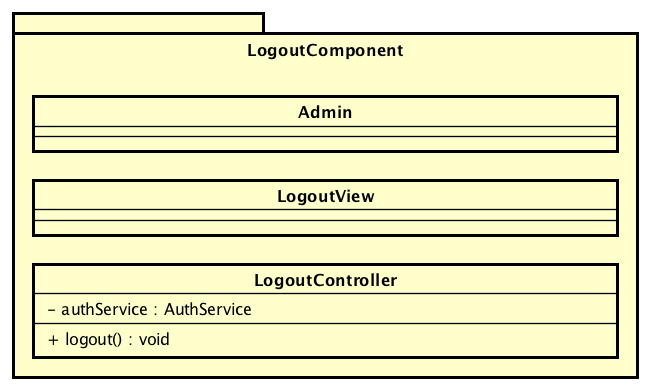
\includegraphics[scale=0.6]{Architettura/Front-End/AdminPage/AdminComponents/LogoutComponent.png}
		\caption{Schema del componente \texttt{Front-End :: AdminPage :: AdminComponents :: LogoutComponent}}
	\end{figure}

			\subparagraph{Descrizione}: Componente che contiene al suo interno la sua view, il suo controller, ed i models di cui necessita
			\subparagraph{Padre}: AdminComponents
	  		\subsubsection{Front-End :: AdminPage :: AdminComponents :: LogoutComponent :: LogoutController}
				\subparagraph{Descrizione}: Componente dedicato all'operazione di logout
				\subparagraph{Costanti}:
				\begin{itemize}
					\item \texttt{authService: AuthService}: Attributo che rappresenta una istanza del service AuthService e ne mette a disposizione i metodi.
				\end{itemize}
				\subsubsection{Front-End :: AdminPage :: AdminComponents :: LogoutComponent :: LogoutView}
				\subparagraph{Descrizione}: View del componente dedicato all'operazione di logout

	\newpage
	\subsection{Front-End :: AdminPage :: AdminComponents :: ManageAdministratorsComponent}
	\begin{figure}[!h]
		\centering
		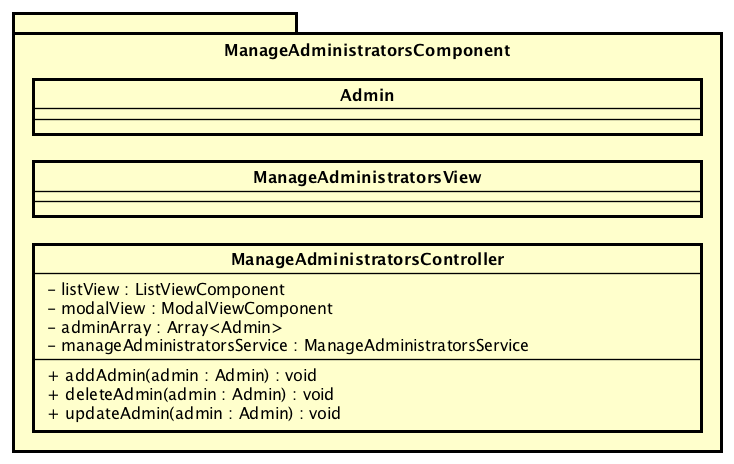
\includegraphics[scale=0.6]{Architettura/Front-End/AdminPage/AdminComponents/ManageAdministratorsComponent.png}
		\caption{Schema del componente \texttt{Front-End :: AdminPage :: AdminComponents :: ManageAdministratorsComponent}}
	\end{figure}

			\subparagraph{Descrizione}: Componente che contiene al suo interno la sua view, il suo controller, ed i models di cui necessita
			\subparagraph{Padre}: AdminComponents
				\subsubsection{Front-End :: AdminPage :: AdminComponents :: ManageAdministratorsComponent :: ManageAdministratorsController}
		      		\subparagraph{Descrizione}: Controller che gestisce la view di ManageAdministrators permettendo ad un SuperAdmin di gestire le informazioni degli altri amministratori
			      	\subparagraph{Attributi}:
					\begin{itemize}
						\item \texttt{listView: ListView}: Attributo che indica la lista che andrà a contenere gli amministratori.
						\item \texttt{modalView: ModalView}: Attributo che indica il modal che conterrà la form per aggiungere o aggiornare un amministratore.
						\item \texttt{adminArray: AdminArray}: Attributo che indica gli amministratori presenti nel sistema.
						\item \texttt{manageAdministratorsService: ManageAdministratorsService}: Attributo che rappresenta una istanza del service ManageAdministratorsService e ne mette a disposizione i metodi.
					\end{itemize}
				\subsubsection{Front-End :: AdminPage :: AdminComponents :: ManageAdministratorsComponent :: ManageAdministratorsView}
					\subparagraph{Descrizione}: View di ManageAdministrators, permette ad un SuperAdmin di gestire le informazioni degli altri amministratori
					\subparagraph{Utilizzo}: View di ManageAdministrators

	\newpage
	\subsection{Front-End :: AdminPage :: AdminComponents :: ManageFirmsComponent}
	\begin{figure}[!h]
		\centering
		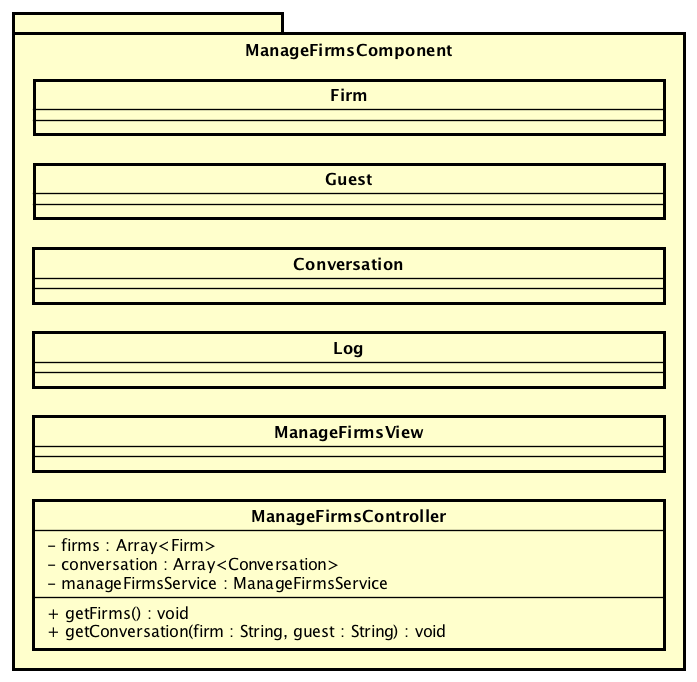
\includegraphics[scale=0.6]{Architettura/Front-End/AdminPage/AdminComponents/ManageFirmsComponent.png}
		\caption{Schema del componente \texttt{Front-End :: AdminPage :: AdminComponents :: ManageFirmsComponent}}
	\end{figure}

			\subparagraph{Descrizione}: Componente che contiene al suo interno la sua view, il suo controller, ed i models di cui necessita
			\subparagraph{Padre}: AdminComponents
				\subsubsection{Front-End :: AdminPage :: AdminComponents :: ManageFirmsComponent :: ManageFirmsController}
					\subparagraph{Descrizione}: Componente utilizzato per la gestione degli oggetti di tipo Firm
					\subparagraph{Attributi}:
					\begin{itemize}
						\item \texttt{firms: Array<Firm>}: Attributo che indica le aziende presenti nel sistema.
						\item \texttt{manageFirmsService: ManageFirmsService}: Attributo che rappresenta una istanza del service ManageFirmsService e ne mette a disposizione i metodi.
					\end{itemize}
				\subsubsection{Front-End :: AdminPage :: AdminComponents :: ManageFirmsComponent :: ManageFirmsView}
					\subparagraph{Descrizione}: View utilizzata per la scelta degli oggetti di tipo Firm


	\newpage
	\subsection{Front-End :: AdminPage :: AdminComponents :: ManageProfileComponent}
	\begin{figure}[!h]
		\centering
		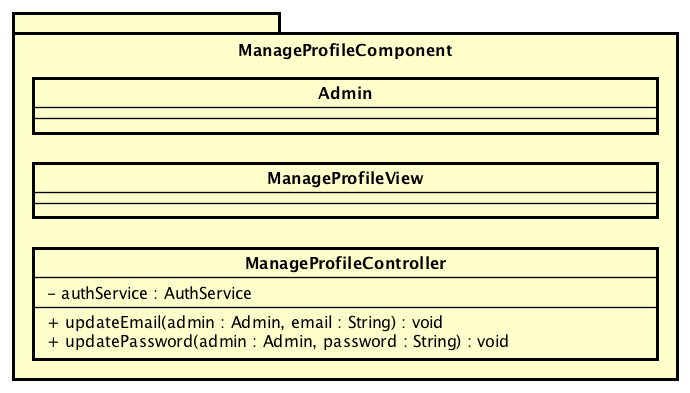
\includegraphics[scale=0.6]{Architettura/Front-End/AdminPage/AdminComponents/ManageProfileComponent.png}
		\caption{Schema del componente \texttt{Front-End :: AdminPage :: AdminComponents :: ManageProfileComponent}}
	\end{figure}
			\subparagraph{Descrizione}: Componente che contiene al suo interno la sua view, il suo controller, ed i models di cui necessita
			\subparagraph{Padre}: AdminComponents
				\subsubsection{Front-End :: AdminPage :: AdminComponents :: ManageProfileComponent :: ManageProfileView}
					\subparagraph{Descrizione}: View di ManageProfile, permette ad un amministratore di gestire il proprio profilo nell'area amministrativa
				\subsubsection{Front-End :: AdminPage :: AdminComponents :: ManageProfileComponent :: ManageProfileController}

					\subparagraph{Descrizione}: Controller che gestisce la view di ManageProfileView permettendo ad un amministratore di gestire il proprio profilo nell'area amministrativa
					\subparagraph{Attributi}:
					\begin{itemize}
						\item \texttt{authService: AuthService}: Attributo che rappresenta una istanza del service AuthService e ne mette a disposizione i metodi.
					\end{itemize}
				\subsubsection{Front-End :: AdminPage :: AdminComponents :: ManageProfileComponent :: ManageProfileView}

					\subparagraph{Descrizione}: View di ManageProfile, permette ad un amministratore di gestire il proprio profilo nell'area amministrativa


	\newpage
	\subsection{Front-End :: AdminPage :: AdminComponents :: ManageQuestionsComponent}
	\begin{figure}[!h]
		\centering
		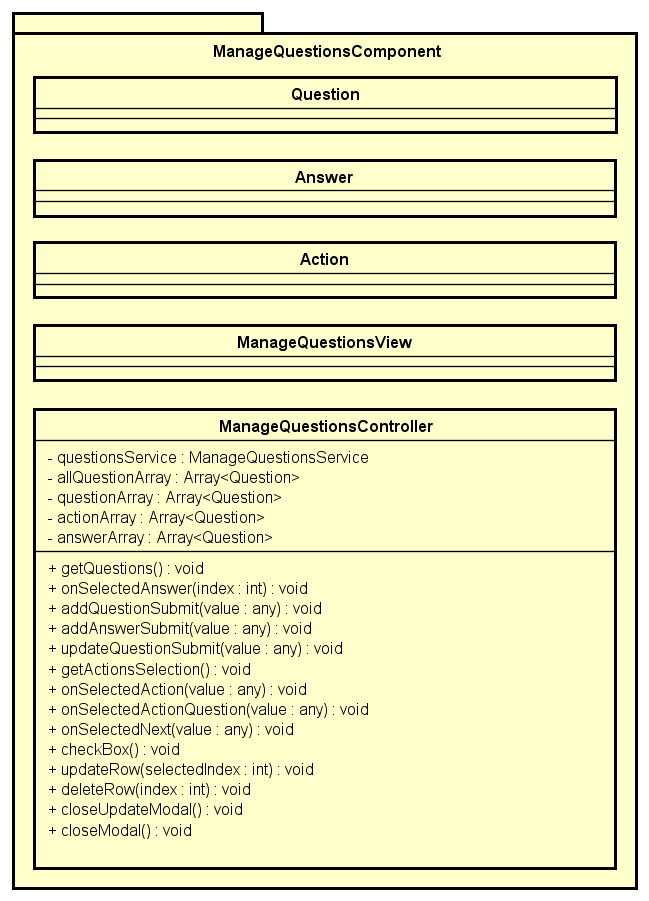
\includegraphics[scale=0.6]{Architettura/Front-End/AdminPage/AdminComponents/ManageQuestionsComponent.png}
		\caption{Schema del componente \texttt{Front-End :: AdminPage :: AdminComponents :: ManageQuestionsComponent}}
	\end{figure}
			\subsubsection{Descrizione}: Componente che contiene al suo interno la sua view, il suo controller, ed i models di cui necessita
			\subsubsection{Padre}: AdminComponents
			      \subsubsection{Front-End :: AdminPage :: AdminComponents :: ManageQuestionsComponent :: ManageQuestionsController}
			      	\subparagraph{Descrizione}: Componente per le domande e interazioni
			      	\subparagraph{Utilizzo}: Componente utilizzato per le domande e interazioni
			      	\subparagraph{Attributi}:
      	      			\begin{itemize}
							\item \texttt{manageQuestionsService : ManageQuestionsService}: Attributo che rappresenta una istanza del service ManageQuestionsService e ne mette a disposizione i metodi.
							\item \texttt{questions: Array<Question, Array<Answer>}: Parametro che indica la lista delle domande presenti nel sistema comprensive delle proprie risposte.
						\end{itemize}
					\subsubsection{Front-End :: AdminPage :: AdminComponents :: ManageQuestionsComponent :: ManageQuestionsView}
						\subparagraph{Descrizione}: View per la gestione di domande e interazioni
						\subparagraph{Utilizzo}: View di ManageQuesitons

	\newpage
	\subsection{Front-End :: AdminPage :: AdminComponentsComponent :: ManageSlack}
	\begin{figure}[!h]
		\centering
		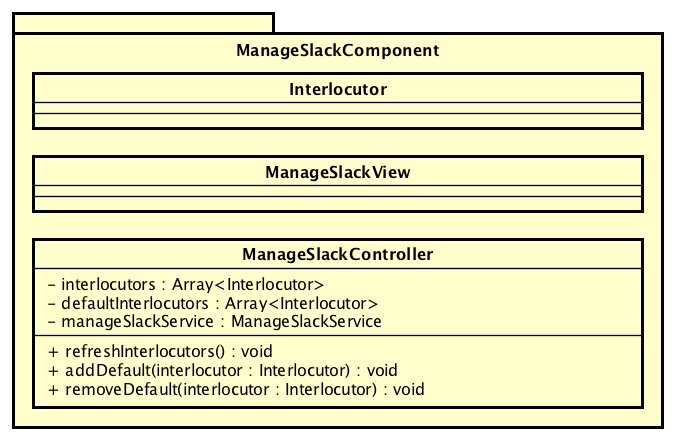
\includegraphics[scale=0.6]{Architettura/Front-End/AdminPage/AdminComponents/ManageSlackComponent.png}
		\caption{Schema del componente \texttt{Front-End :: AdminPage :: AdminComponents :: ManageSlackComponent}}
	\end{figure}
			\subparagraph{Descrizione}: Componente che contiene al suo interno la sua view, il suo controller, ed i models di cui necessita
			\subparagraph{Padre}: AdminComponents
			      \subsubsection{Front-End :: AdminPage :: AdminComponents :: ManageSlackComponent :: ManageSlackController}
			      	\subparagraph{Descrizione}: Componente per la gestione dei canali Slack
			      	\subparagraph{Utilizzo}: Componente per la gestione dei canali Slack
			      	\subparagraph{Attributi}:
					\begin{itemize}
						\item \texttt{defaultInterlocutors: Array<Interlocutor>}: Attributo che indica gli interlocutori presenti nel sistema che fanno parte della lista di default del canale \#azienda.
						\item \texttt{interlocutor: Array<Interlocutor>}: Attributo che indica gli interlocutori presenti nel sistema.
						\item \texttt{manageSlackService: ManageSlackService}: Attributo che rappresenta una istanza del service ManageSlackService e ne mette a disposizione i metodi.
					\end{itemize}
		      	\subsubsection{Front-End :: AdminPage :: AdminComponents :: ManageSlackComponent :: ManageSlackView}
					\subparagraph{Descrizione}: View del componente per la gestione dei canali Slack
					\subparagraph{Utilizzo}: View di ManageSlack

	\newpage
	\subsection{Front-End :: AdminPage :: AdminComponents :: UpdatePasswordComponent}
	\begin{figure}[!h]
		\centering
		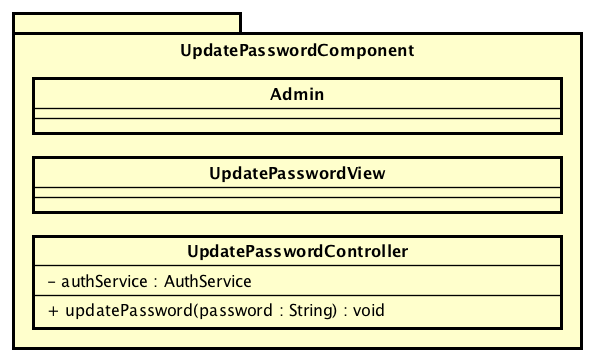
\includegraphics[scale=0.6]{Architettura/Front-End/AdminPage/AdminComponents/UpdatePasswordComponent.png}
		\caption{Schema del componente \texttt{Front-End :: AdminPage :: AdminComponents :: UpdatePasswordComponent}}
	\end{figure}

			\subparagraph{Descrizione}: Componente che contiene al suo interno la sua view, il suo controller, ed i models di cui necessita
			\subparagraph{Padre}: AdminComponents
				\subsubsection{Front-End :: AdminPage :: AdminComponents :: UpdatePasswordComponent :: UpdatePasswordController}
					\subparagraph{Descrizione}: Controller che gestisce la view di UpdatePasswordView permettendo ad un amministratore di effettuare l'aggiornamento della propria password previa email ricevuta nella propria casella di posta
					\subparagraph{Utilizzo}: Metodo utilizzato per gestire il cambio della propria password da parte di un Admin
					\subparagraph{Attributi}:
					\begin{itemize}
						\item \texttt{authService: AuthService}: Attributo che rappresenta una istanza del service AuthService e ne mette a disposizione i metodi.
					\end{itemize}
				\subsubsection{Front-End :: AdminPage :: AdminComponents :: UpdatePasswordComponent :: UpdatePasswordView}

		      		\subparagraph{Descrizione}: View di UpdatePassword, permette ad un amministratore di effettuare l'aggiornamento della propria password previa email ricevuta nella propria casella di posta
			      	\subparagraph{Utilizzo}: View di UpdatePasword


	\newpage
	\subsection{Front-End :: AdminPage :: AdminComponents :: ListViewComponent}
	\begin{figure}[!h]
		\centering
		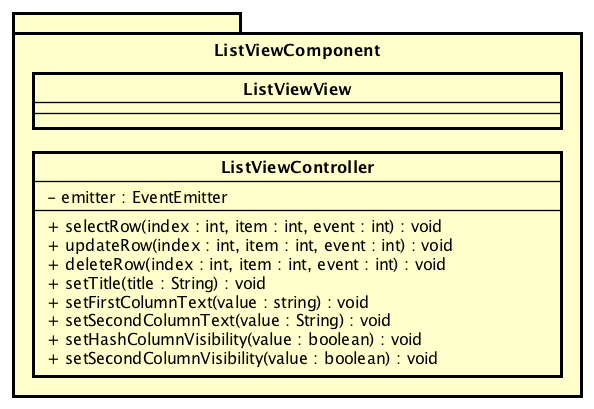
\includegraphics[scale=0.6]{Architettura/Front-End/AdminPage/AdminComponents/ListViewComponent.png}
		\caption{Schema del componente \texttt{Front-End :: AdminPage :: AdminComponents :: ListViewComponent}}
	\end{figure}

			\subparagraph{Descrizione}: Componente che contiene al suo interno la sua view, il suo controller, ed i models di cui necessita
			\subparagraph{Padre}: AdminComponents
			      \subsubsection{Front-End :: AdminPage :: AdminComponents :: ListViewComponent :: ListViewController}
			      	\subparagraph{Descrizione}: Controller che gestisce la view di ListViewComponent permettendo di gestire la lista dell'area amministrativa in tutti i contesti in qui viene chiamata in causa
			      	\subparagraph{Utilizzo}: Verrà utilizzato dall'amministratore per gestire le liste presenti nell'area amministrativa
			      	\subparagraph{Attributi}:
			      	      \begin{itemize}
			      	      	\item \texttt{emitter: EventEmitter<any>}: Attributo che rappresenta un'istanza di EventEmitter e ne mette a disposizione i relativi metodi.
			      	      \end{itemize}
			      \subsubsection{Front-End :: AdminPage :: AdminComponents :: ListViewComponent :: ListViewView}
			      	\subparagraph{Descrizione}: View di ListViewComponent, permette di gestire la lista dell'area amministrativa
			      	\subparagraph{Utilizzo}: View di ListViewComponent
\newpage
	\subsection{Front-End :: AdminPage :: AdminComponents :: ModalViewComponent}
	\begin{figure}[!h]
		\centering
		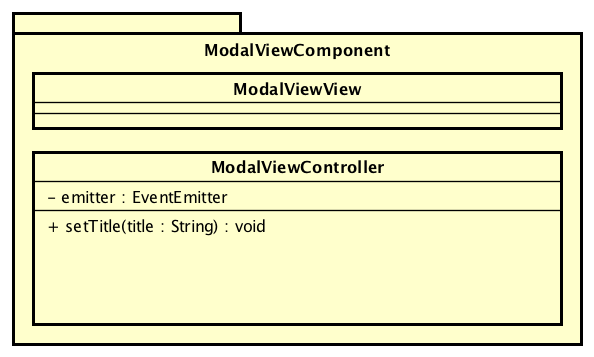
\includegraphics[scale=0.6]{Architettura/Front-End/AdminPage/AdminComponents/ModalViewComponent.png}
		\caption{Schema del componente \texttt{Front-End :: AdminPage :: AdminComponents :: ModalViewComponent}}
	\end{figure}

			\subparagraph{Descrizione}: Componente che contiene al suo interno la sua view, il suo controller, ed i models di cui necessita
			\subparagraph{Padre}: AdminComponents
				\subsubsection{Front-End :: AdminPage :: AdminComponents :: ModalViewComponent :: ModalViewController}
					\subparagraph{Descrizione}: Controller che gestisce la view di ModalViewComponent permettendo di gestire il modal dell'area amministrativa in tutti i contesti in qui viene chiamato in causa
					\subparagraph{Utilizzo}: Verrà utilizzato dall'amministratore per gestire i form atti ad inserire nuove istanze di un oggetto presenti nell'area amministrativa
					\subparagraph{Attributi}:
					      \begin{itemize}
			      	      	\item \texttt{emitter: EventEmitter<any>}: Attributo che rappresenta un'istanza di EventEmitter e ne mette a disposizione i relativi metodi.
			      	      \end{itemize}
				\subsubsection{Front-End :: AdminPage :: AdminComponents :: ModalViewComponent :: ModalViewController}
					\subparagraph{Descrizione}: View di ModalViewComponent, permette di gestire il modal dell'area amministrativa
					\subparagraph{Utilizzo}: View di ModalViewComponent


	\newpage
	\subsection{Front-End :: AdminPage :: AdminServices}

			\subparagraph{Descrizione}: Package che fornisce tutti i servizi utilizzabili da un amministratore ed un super amministratore nella view del Front-End
			\subparagraph{Padre}: AdminPage

				\subsubsection{Front-End :: AdminPage :: AdminServices :: ManageAdministratorsService}
				\begin{figure}[!h]
					\centering
					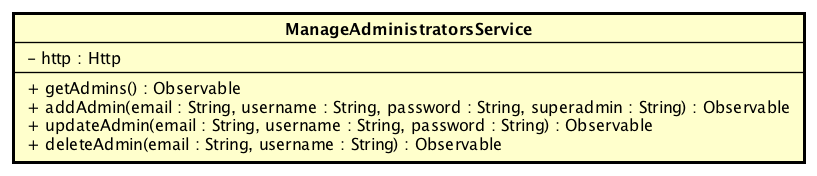
\includegraphics[scale=0.6]{Architettura/Front-End/AdminPage/AdminServices/ManageAdministratorsService.png}
					\caption{Schema del service \texttt{Front-End :: AdminPage :: AdminServices :: ManageAdministratorsService}}
				\end{figure}

					\subparagraph{Descrizione}: Servizi per i componenti del client dell'Admin e del SuperAdmin.
					\subparagraph{Utilizzo}: Gestione servizi Admin e SuperAdmin.
					\subparagraph{Attributi}:
					\begin{itemize}
						\item \texttt{http: Http}: Attributo che rappresenta un'istanza di Http e ne mette a disposizione i relativi metodi.
					\end{itemize}
\newpage
		      	\subsubsection{Front-End :: AdminPage :: AdminServices :: ManageFirmsService}
				\begin{figure}[!h]
					\centering
					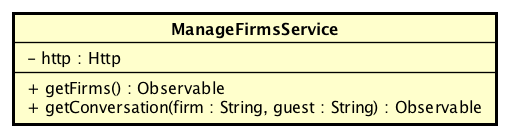
\includegraphics[scale=0.6]{Architettura/Front-End/AdminPage/AdminServices/ManageFirmsService.png}
					\caption{Schema del service \texttt{Front-End :: AdminPage :: AdminServices :: ManageFirmsService}}
				\end{figure}
			      	\subparagraph{Descrizione}: Gestione servizi per i componenti client che si occupano delle aziende.
			      	\subparagraph{Utilizzo}: Utilizzato per gestire le aziende.
			      	\subparagraph{Attributi}:
      	      		\begin{itemize}
						\item \texttt{http: Http}: Attributo che rappresenta un'istanza di Http e ne mette a disposizione i relativi metodi.
	      	      	\end{itemize}
\newpage
				\subsubsection{Front-End :: AdminPage :: AdminServices :: ManageQuestionsService}
				\begin{figure}[!h]
					\centering
					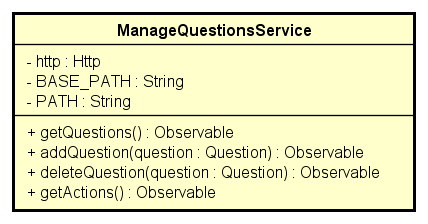
\includegraphics[scale=0.6]{Architettura/Front-End/AdminPage/AdminServices/ManageQuestionsService.png}
					\caption{Schema del service \texttt{Front-End :: AdminPage :: AdminServices :: ManageQuestionsService}}
				\end{figure}

					\subparagraph{Descrizione}: Classe che fornisce funzionalità per la gestione delle domande e delle interazioni collegate ad esse
					\subparagraph{Utilizzo}: Utilizzata per operazioni di gestione delle domande e relative interazioni
					\subparagraph{Attributi}:
			      	\begin{itemize}
						\item \texttt{http: Http}: Attributo che rappresenta un'istanza di Http e ne mette a disposizione i relativi metodi.
			      	\end{itemize}
\newpage

     	 		\subsubsection{Front-End :: AdminPage :: AdminServices :: ManageSlackService}
				\begin{figure}[!h]
					\centering
					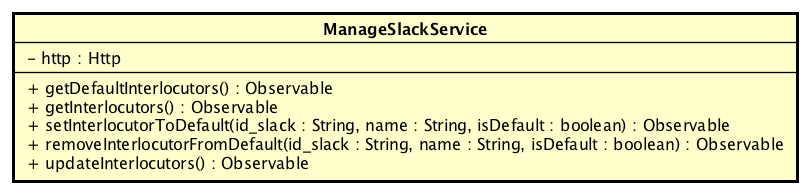
\includegraphics[scale=0.6]{Architettura/Front-End/AdminPage/AdminServices/ManageSlackService.png}
					\caption{Schema del service \texttt{Front-End :: AdminPage :: AdminServices :: ManageSlackService}}
				\end{figure}

				\subsubsection{Descrizione}: Gestione servizi lato client dei componenti che si interfacciano ai servizi di Slack.
				\subsubsection{Utilizzo}: Utilizzato per gestire i servizi di interfaccia ai servizi di Slack.
				\subsubsection{Attributi}:
				\begin{itemize}
					\item \texttt{http: Http}: Attributo che rappresenta un'istanza di Http e ne mette a disposizione i relativi metodi.
				\end{itemize}
\newpage
		      	\subsubsection{Front-End :: AdminPage :: AdminServices :: AuthService}
				\begin{figure}[!h]
					\centering
					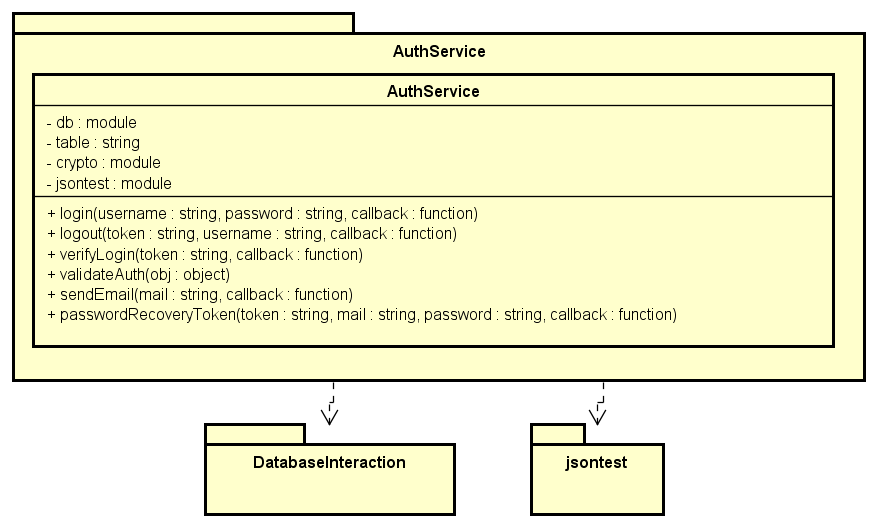
\includegraphics[scale=0.6]{Architettura/Front-End/AdminPage/AdminServices/AuthService.png}
					\caption{Schema del service \texttt{Front-End :: AdminPage :: AdminServices :: AuthService}}
				\end{figure}

				\subparagraph{Descrizione}: Classe che fornisce servizi per effettuare operazioni di autenticazione nel client dell'Admin e del SuperAdmin
				\subparagraph{Utilizzo}: Utilizzata quando un amministratore o un super amministratore effettua operazioni di autenticazione nell'interfaccia
				\subparagraph{Attributi}:
				\begin{itemize}
					\item \texttt{http: Http}: Attributo che rappresenta un'istanza di Http e ne mette a disposizione i relativi metodi.
				\end{itemize}
	\newpage
	\subsection{Front-End :: GuestPage}
	\begin{figure}[!h]
		\centering
		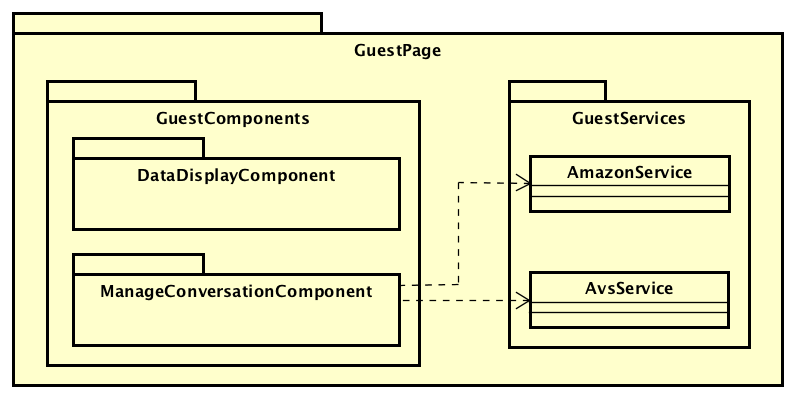
\includegraphics[scale=0.6]{Architettura/Front-End/GuestPage/GuestPage.png}
		\caption{Schema del componente \texttt{Front-End :: GuestPage}}
	\end{figure}

			\subparagraph{Descrizione}: Package dedicato alla parte d'interfaccia client disponibile all'ospite
			\subparagraph{Padre}: Front-End
			\subparagraph{Package contenuti}:
			\begin{itemize}
				\item Front-End :: GuestPage :: GuestComponents: Package dedicato alla parte view e controller dell'interfaccia ospite
				\item Front-End :: GuestPage :: GuestServices: Package dedicato ai servizi resi disponibili a GuestComponents
			\end{itemize}


	\newpage
	\subsection{Front-End :: GuestPage :: GuestComponents}

			\subparagraph{Descrizione}: Package dedicato alla parte view e controller dell'interfaccia ospite
			\subparagraph{Padre}: GuestPage
			\subparagraph{Package contenuti}:
			\begin{itemize}
				\item Front-End :: GuestPage :: GuestComponents :: ManageConversationComponent: Componente che contiene al suo interno la sua view, il suo controller, ed i models di cui necessita
				\item Front-End :: GuestPage :: GuestComponents :: DataDisplayComponent: Componente che contiene al suo interno la sua view, il suo controller, ed i models di cui necessita
			\end{itemize}

	\newpage
	\subsection{Front-End :: GuestPage :: GuestComponents :: ManageConversationComponent}
	\begin{figure}[!h]
		\centering
		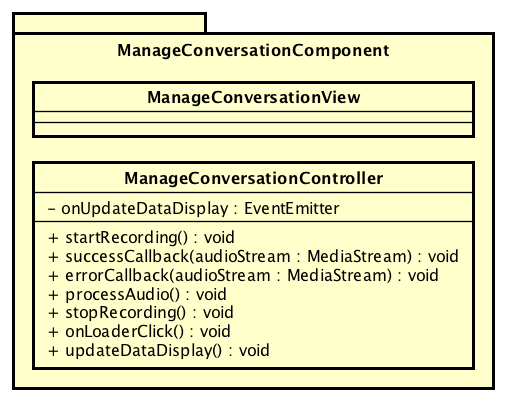
\includegraphics[scale=0.7]{Architettura/Front-End/GuestPage/GuestComponents/ManageConversationComponent.png}
		\caption{Schema del componente \texttt{Front-End :: GuestPage :: GuestComponents :: ManageConversationComponent}}
	\end{figure}

			\subparagraph{Descrizione}: Componente che contiene al suo interno la sua view, il suo controller, ed i models di cui necessita
			\subparagraph{Padre}: GuestComponents
			      
			\subsubsection{Front-End :: GuestPage :: GuestComponents :: ManageConversationComponent :: ManageConversationController}

				\subparagraph{Descrizione}: Classe che si occupa di gestire la conversazione tra ospite e sistema
				\subparagraph{Utilizzo}: Sarà utilizzata per permettere la conversazione tra ospite e Assistente Virtuale
				\subparagraph{Attributi}:
				\begin{itemize}
					\item \texttt{onUpdateDataDisplay : EventEmitter<any>}: Attributo che rappresenta un'istanza di EventEmitter e ne mette a disposizione i relativi metodi.
				\end{itemize}
			\subsubsection{Front-End :: GuestPage :: GuestComponents :: ManageConversationComponent :: ManageConversationView}

				\subparagraph{Descrizione}: Classe utilizzata per visualizzare la conversazione tra ospite e AV
				\subparagraph{Utilizzo}: View di ManageConversationComponent

	\newpage
	\subsection{Front-End :: GuestPage :: GuestComponents :: DataDisplayComponent}
	\begin{figure}[!h]
		\centering
		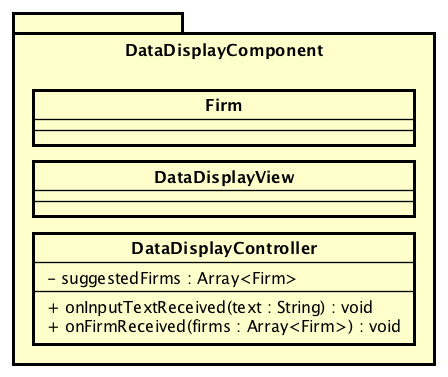
\includegraphics[scale=0.7]{Architettura/Front-End/GuestPage/GuestComponents/DataDisplayComponent.png}
		\caption{Schema del componente \texttt{Front-End :: GuestPage :: GuestComponents :: DataDisplayComponent}}
	\end{figure}

			\subparagraph{Descrizione}: Componente che contiene al suo interno la sua view, il suo controller, ed i models di cui necessita
			\subparagraph{Padre}: GuestComponents
			
			\subsubsection{Front-End :: GuestPage :: GuestComponents :: DataDisplayComponent :: DataDisplayController}
				\subparagraph{Descrizione}: Classe contenente tutti i metodi necessari a mostrare a schermo informazioni utili all'ospite
				\subparagraph{Utilizzo}: Verrà utilizzata per fornire informazioni all'utente o ospite
				\subparagraph{Attributi}:
				\begin{itemize}
					\item \texttt{sugestedFirms: Array<Firm>}: Attributo di appoggio che indica un array di aziende da mostrare a video all'ospite
				\end{itemize}
			\subsubsection{Front-End :: GuestPage :: GuestComponents :: DataDisplayComponent :: DataDisplayView}

				\subparagraph{Descrizione}: Classe contenente tutti i metodi necessari a mostrare a schermo informazioni utili all'utente o ospite
				\subparagraph{Utilizzo}: View di DataDisplayComponent

	\newpage
	\subsection{Front-End :: GuestPage :: GuestServices}
	
			\subparagraph{Descrizione}: Package dedicato ai servizi resi disponibili agli ospiti 
			\subparagraph{Padre}: GuestPage
		
			\subsubsection{Front-End :: GuestPage :: GuestServices :: AmazonService}
			\begin{figure}[!h]
				\centering
				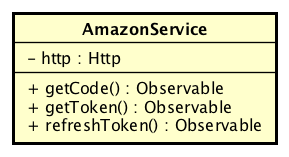
\includegraphics[scale=0.6]{Architettura/Front-End/GuestPage/GuestServices/AmazonService.png}
				\caption{Schema del service \texttt{Front-End :: GuestPage :: GuestServices :: AmazonService}}
			\end{figure}

			\subparagraph{Descrizione}: Contiene i servizi necessari ad effettuare l'autenticazione ad Amazon ed iniziare ad utilizzare Alexa Voice Service
			\subparagraph{Utilizzo}: Servizi per i components dell'interfaccia ospite.
			\subparagraph{Attributi}:
			\begin{itemize}
				\item \texttt{http: Http}: Attributo che rappresenta un'istanza di Http e ne mette a disposizione i relativi metodi.
			\end{itemize}

\newpage
			\subsubsection{Front-End :: GuestPage :: GuestServices :: AvsService}
			\begin{figure}[!h]
				\centering
				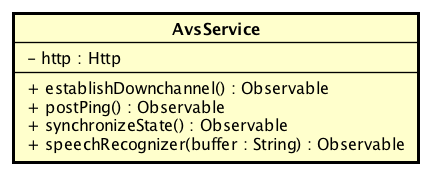
\includegraphics[scale=0.6]{Architettura/Front-End/GuestPage/GuestServices/AvsService.png}
				\caption{Schema del service \texttt{Front-End :: GuestPage :: GuestServices :: AvsService}}
			\end{figure}

				\subparagraph{Descrizione}: Contiene i servizi necessari ad effettuare le chiamate alle API di Alexa Voice Service
				\subparagraph{Utilizzo}: Servizi per i components dell'interfaccia ospite.
				\subparagraph{Attributi}:
				\begin{itemize}
					\item \texttt{http: Http}: Attributo che rappresenta un'istanza di Http e ne mette a disposizione i relativi metodi.
				\end{itemize}
\end{document}